\section {Analysis}\label{sec:analysis}

\begin{figure*}[t]
    \centering
    \begin{subfigure}[b]{0.48\textwidth}
        \centering
        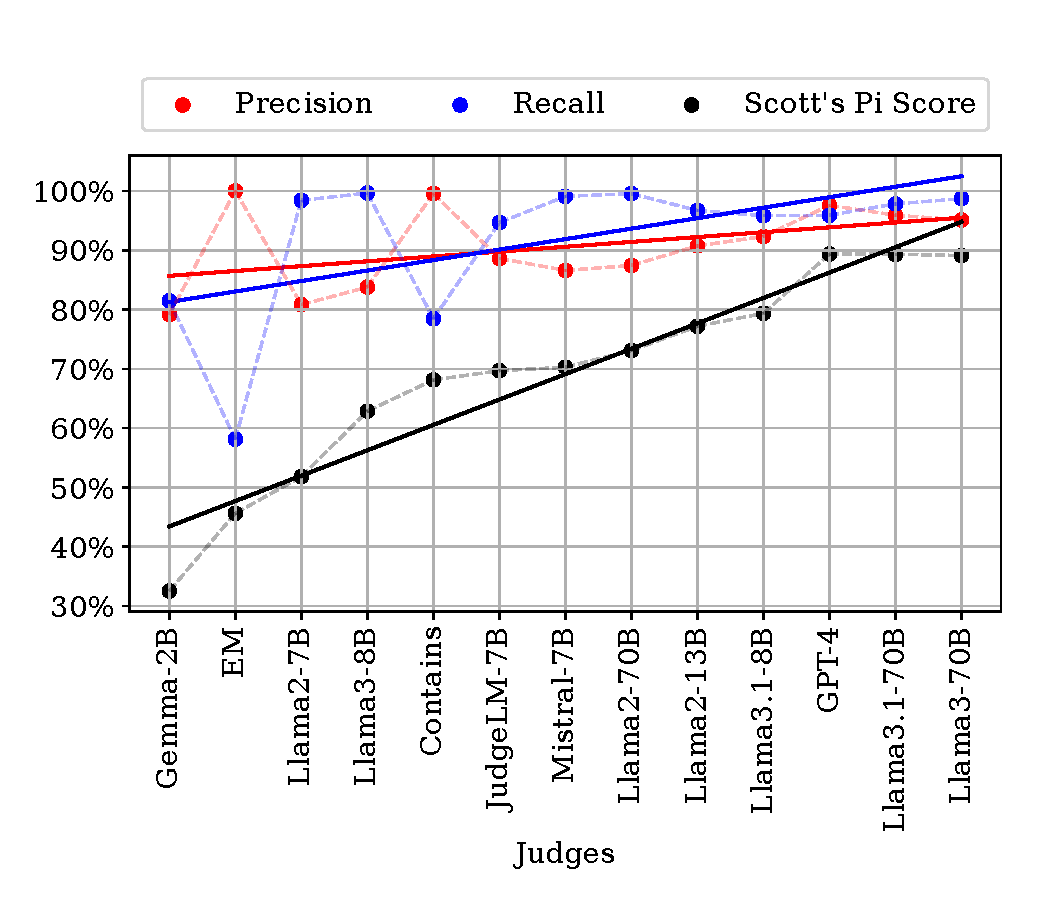
\includegraphics[width=\linewidth]{figures/PrecisionRecall_V6.pdf}
        \vspace{-6mm}
        \caption{}
        \vspace{-2mm}
        \label{fig:precisionrecall}
    \end{subfigure}
    \hfill
    \centering
    \begin{subfigure}[b]{0.51\textwidth}
        \centering
        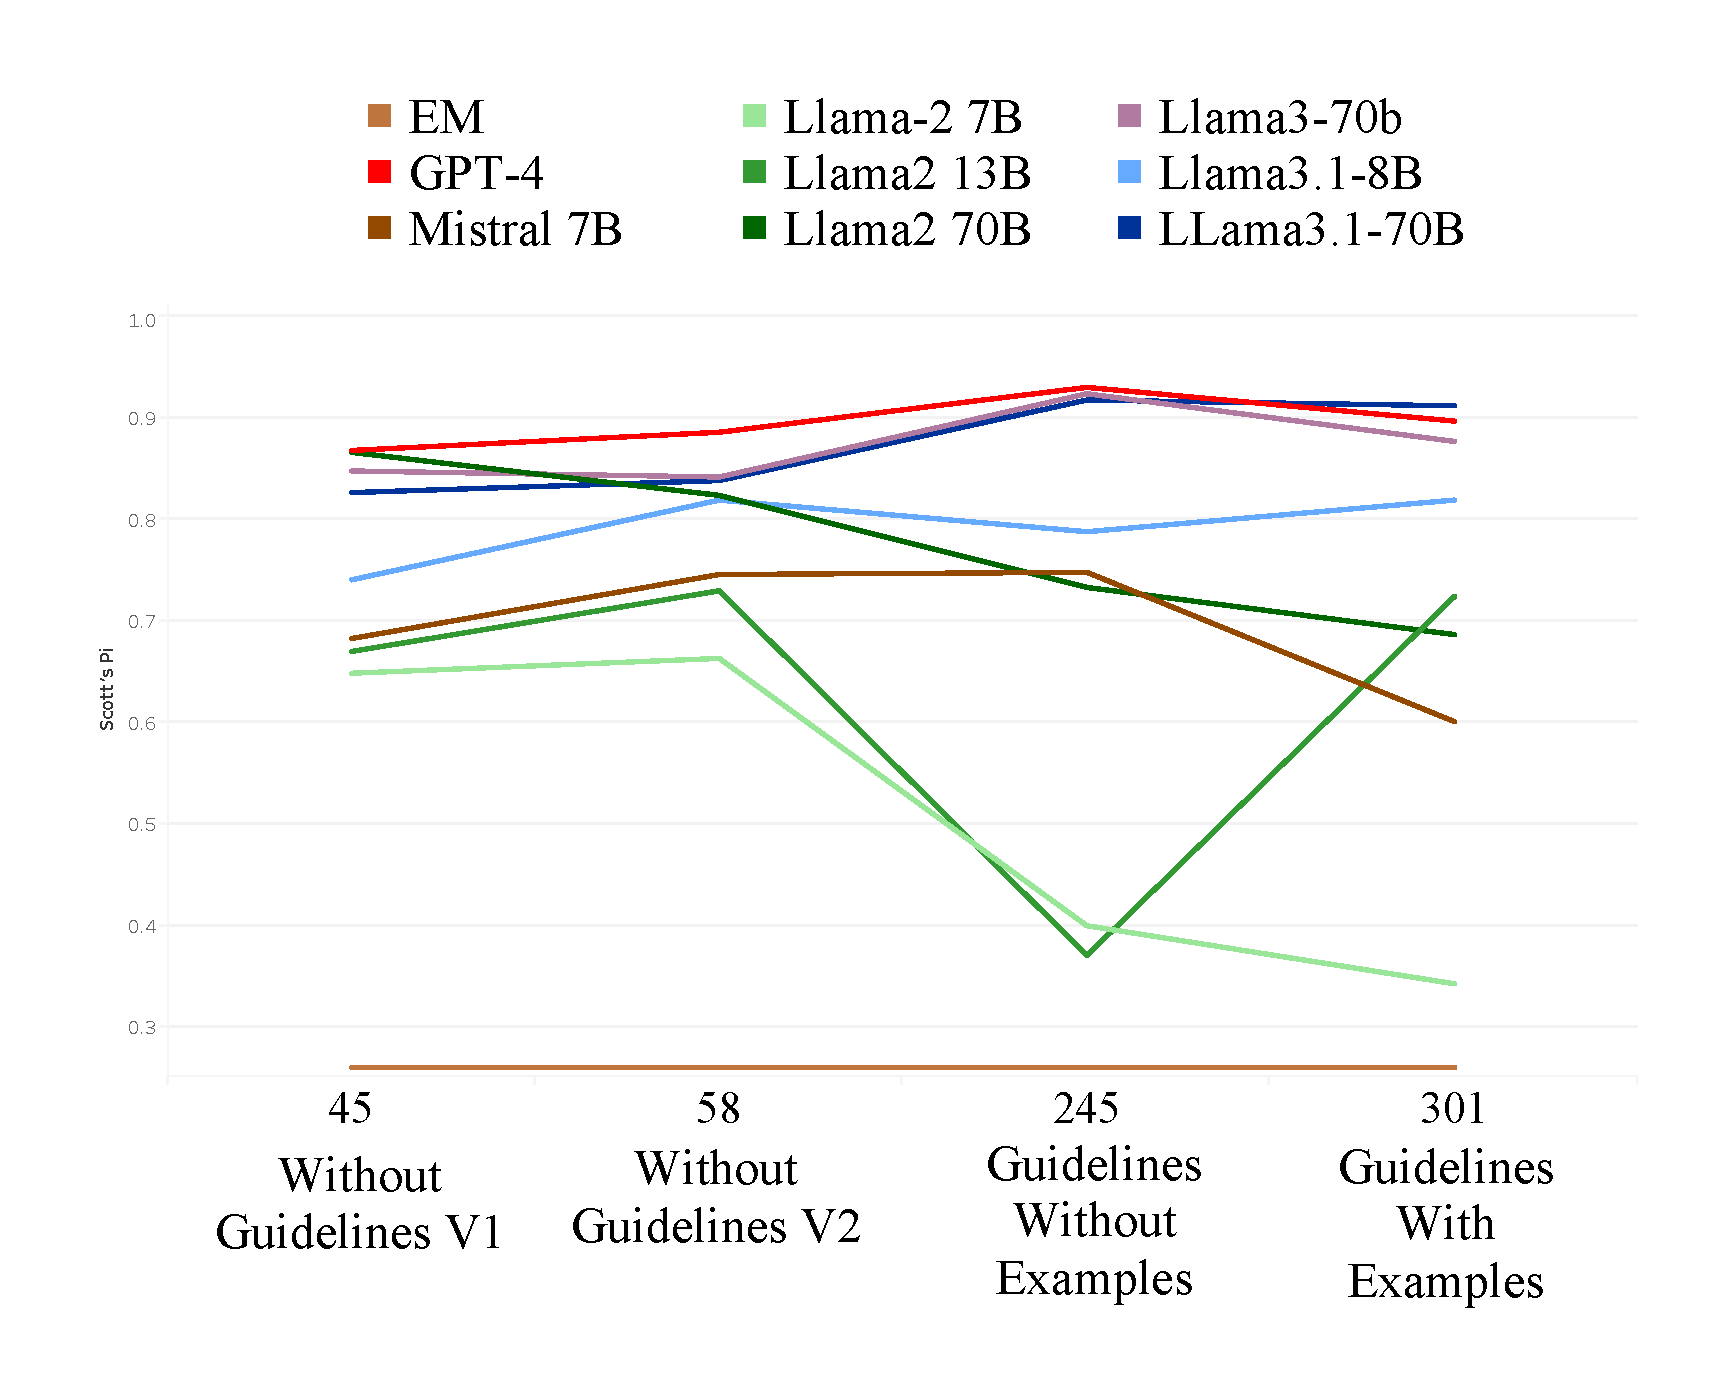
\includegraphics[width=\linewidth]{figures/TooMuchInfo.pdf}
        \vspace{-6mm}
        \caption{}
        \vspace{-2mm}
        \label{fig:TooMuchInfo}
    \end{subfigure}
    
% This adds space between the subfigures
    \caption{\textbf{Precision, recall and prompt sensitivity.} (a) Recall and precision improve with increasing human alignment (\( R^2 \) = 0.31 and \( R^2 \) = 0.21, respectively). %(\( R^2 \) = 0.91). 
    (b) \scottspi scores for judges across different instructions. 
    }
\end{figure*}

\begin{table*}[t]
% \captionsetup{skip=8pt} % Adjust space between table and caption
\resizebox{\textwidth}{!}{
    \begin{tabular}{lllllll}
        \textbf{Error code} & \textbf{Explanation} & \textbf{Example} & \textbf{Proportion} & \textbf{GPT-4 recall} & \textbf{Llama-3 70B recall}\\ 
        \toprule\toprule
        \textbf{Incorrect entity} & \specialcell{Response refers to a wrong entity} & \specialcell{\texttt{Henry VII, James I, Edward VI,} \\ \texttt{Mary I and Elizabeth I}} & 86.9\% & \textbf{98.3\%} & \textbf{96.6\%}\\
        \hline
        \textbf{Under-specified} & \specialcell{Response contains only part \\ of the answer} & \specialcell{\texttt{Henry VII, Henry VIII, Edward,} \\ \texttt{Mary, and Elizabeth}} & 37.3\% & 33.9\% & 23.3\% \\
        \hline
        \textbf{Too few entities} & \specialcell{Response contains too few entities} & \specialcell{\texttt{Henry VII, Edward VI,} \\ \texttt{Mary I and James I}} & 2.47\% & \textbf{80.0\%} & 60.0\%\\
        \hline
        \textbf{Too many entities} & \specialcell{Response contains too many entities} & \specialcell{\texttt{Henry VII, Henry VIII, Edward VI,} \\ \texttt{Mary I, James I, and Elizabeth I}} & 2.7\% & \textbf{90.1\%} & \textbf{90.1\%} \\
        \hline
        \textbf{Other} & \specialcell{Response is incorrect but cannot \\ be put into any of the above buckets} & \specialcell{\texttt{I'm sorry but I do not know the} \\ \texttt{answer to that question}} & 1.23\% & 20.0\% & 40.0\% \\
        \bottomrule
    \end{tabular}
    }
     \caption{\textbf{Error analysis for \judge{GPT-4} and \judge{Llama-3 70B} judges.} 
     %Error codes used to identify the types of errors made by \evaluatormodels when answering questions. 
     The example question is \textit{``Excluding Lady Jane Grey, who were the five monarchs of the House of Tudor?''}, the correct answer \textit{``Henry VII, Henry VIII, Edward VI, Mary I and Elizabeth I''} (in any order).}
     \label{table:error_codes}
\end{table*}

To better understand the \judgemodels, we conduct multiple case studies aimed at identifying common errors and vulnerabilities in the judges we investigate.
Specifically, we study their precision and recall and error types (\cref{sec:analysis:subsec:precision_recall}), their sensitivity to the instruction prompt prompt (\cref{sec:analysis:subsec:instructions}), how they respond to controlled resposes of specific types (\cref{sec:analysis:subsec:judge-ability}), and the extent to which they have a \textit{leniency bias} (\cref{sec:leniency-bias}).
% We study the precision and recall of the \judgemodels and their ability to recall specific error types (\cref{sec:analysis:subsec:precision_recall}), how sensitive \judgemodels are to the length of prompts and the clarity of guidelines (\cref{sec:analysis:subsec:instructions}), ability of judges to evaluate controlled responses (\cref{sec:analysis:subsec:judge-ability}), the leniency of \judgemodels in grading (\cref{sec:leniency-bias}) and the difference in evaluation of base and chat \evaluatormodels (\cref{app:BaseVsChatSupp}).
%\dieuwke{insert rest of the results}.

\subsection{Better aligned models: Precision and recall gains with error spotlights}
\label{sec:analysis:subsec:precision_recall}

We first examine the precision and recall of the \judgemodels. As shown in \cref{fig:precisionrecall}, both metrics increase moderately with alignment. \cref{fig:confusionmatrix} reveals a similar trend, with a clearer distribution of false positives and negatives. True positives remain consistent across varying judge quality, whereas true negatives exhibit a slight decline as judge quality decreases. Notably, a reduction in judge quality leads to an increase in false positives.

% True positives remain stable across many judges, while true negatives decrease as judge quality drops, indicating it's easier to identify correct answers.

Next, we analyze the errors made by \judgemodels by manually annotating 900 outputs from \eval{Llama-7B Base}, focusing on top performers \judge{\gpt} and \judge{Llama-3;70B}. We categorize error types and determine how often they are correctly judged as incorrect. The results in \cref{table:error_codes} show that both \judge{\gpt} and \judge{Llama-3;70B} excel at identifying answers referring to incorrect entities or containing too many entities. Under-specified and incorrect answers are more challenging, with \judge{\gpt} performing better on answers with fewer entities than \judge{Llama-3;70B}.

% We first investigate the precision and recall of the \judgemodels. 
% Maintaining the ordering of \cref{fig:llmalignment}, we plot both in \cref{fig:precisionrecall}. 
% We can see that both precision and recall exhibit a moderate increasing trend as alignment increases. 
% In \cref{fig:confusionmatrix}, we observe a similar pattern, though with a clearer picture on the distribution of false positives and negatives.
% Specifically, we see that the number of true positives is quite stable across many judges.
% The true negatives, instead, drop off quickly as the judge quality decreases, suggesting it is generally easier to judge answers that are correct.

% there is a similar pattern to observe; a sharp decline in false positives initially, along with a gradual decline in false negatives.

% It can be seen that the precision shows moderate r observable trend with increasing alignment, which can be further observed in \cref{fig:confusionmatrix}.
% The recall, \sout{on the other hand}, shows an increasing trend, with more aligned models having comparatively fewer false negatives.

% \begin{figure}[h]
%     \centering
%         \includegraphics[width=\linewidth]{figures/ConfusionMatrixV2.png}
%         \caption{Judge performance \& error rate with increasing human alignment }
%         \label{fig:confusionmatrix}
% \end{figure}

% \subsection{What types of errors do \judgemodels recall?}\label{sec:analysis:subsec:error_analysis}

% Next, we analyse the types of errors made by the \judgemodels by manually annotating 900 outputs from \eval{Llama-7B Base} with error codes, focusing on the top performers \judge{\gpt} and \judge{Llama-3\;70B}.
% We then determine the percentage of each error type that are correctly judged to be incorrect by these two models.
% The results are shown in \cref{table:error_codes}, where it can be observed that both \judge{\gpt} and \judge{Llama-3 70B} have a good error recall when the answers refer to an incorrect entity, or when too many entities are present.
% Under-specified and otherwise incorrect answers are most challenging for both judges, while answers with too few entities are judged relatively accurately by \judge{GPT-4} but less accurately by \judge{Llama-3 70B}.
% However, the judge can mark answers as correct when they are only \textit{partially} correct (i.e.\ when they have too few or under-specified entities), which appears to be a source of misalignment between humans and \judgemodels.

% \setlength{\textfloatsep}{10pt}
% From this case study, we can see that 87\% of incorrect responses were because of knowledge gap of evaluation model. 
% Using GPT-4 Judge LLM, we evaluate each of the responses and then calculate the recall of each error code. From \cref{fig:recallfpr}, we observe that GPT-4 accurately recalls incorrect entities, too many entities, and too few entities. 
% However, GPT-4's recall drops to 20\% - 20\% for underspecified and other error codes indicating that it may be lenient with such error codes.
% 
% \begin{figure}[h]
%     \begin{subfigure}[b]{0.49\linewidth}
%         \centering
%         \includegraphics[width=\linewidth]{figures/ErrorCodeAnalysisV2.png}
%         \caption{\judge{GPT-4}}
%         \label{fig:recallfpr}
%     \end{subfigure}
%     \begin{subfigure}[b]{0.49\linewidth}
%         \centering
%         \includegraphics[width=\linewidth]{figures/ErrorCodeAnalysisV2.png}
%         \caption{\judge{Llama3-70B-Chat}}
%         \label{fig:recallfpr}
%     \end{subfigure}
%     \caption{Recall of specific errors by \judge{GPT-4} and \judge{Llama3-70B-chat}. 
%     `Proportion' indicates how many of the observed errors were of that specific type.
%     \dieuwke{Create Llama 3 plot on the right.}}
% \end{figure}

% \begin{figure}
%     \centering
%     \begin{subfigure}[b]{0.42\textwidth}
%         \includegraphics[width=\textwidth]{figures/ErrorCodeAnalysisV2}
%         \caption{}\label{fig:generalisation_over_time_c}
%     \end{subfigure}
%     \caption{}\label{fig:generalisation_over_time}
% \end{figure}

% \begin{figure}[H]
%     \centering
%     \begin{minipage}[t]{\textwidth}
%         \centering
%         \includegraphics[width=1\textwidth, height=\textheight, keepaspectratio]{figures/TooMuchInfo_Scaled.pdf}
%         \caption{Cohen's Kappa score (human alignment) vs prompt token size for judge LLMs}
%         \label{fig:TooMuchInfo}
%     \end{minipage}
% \end{figure}

\begin{figure*}[t]
    \centering
    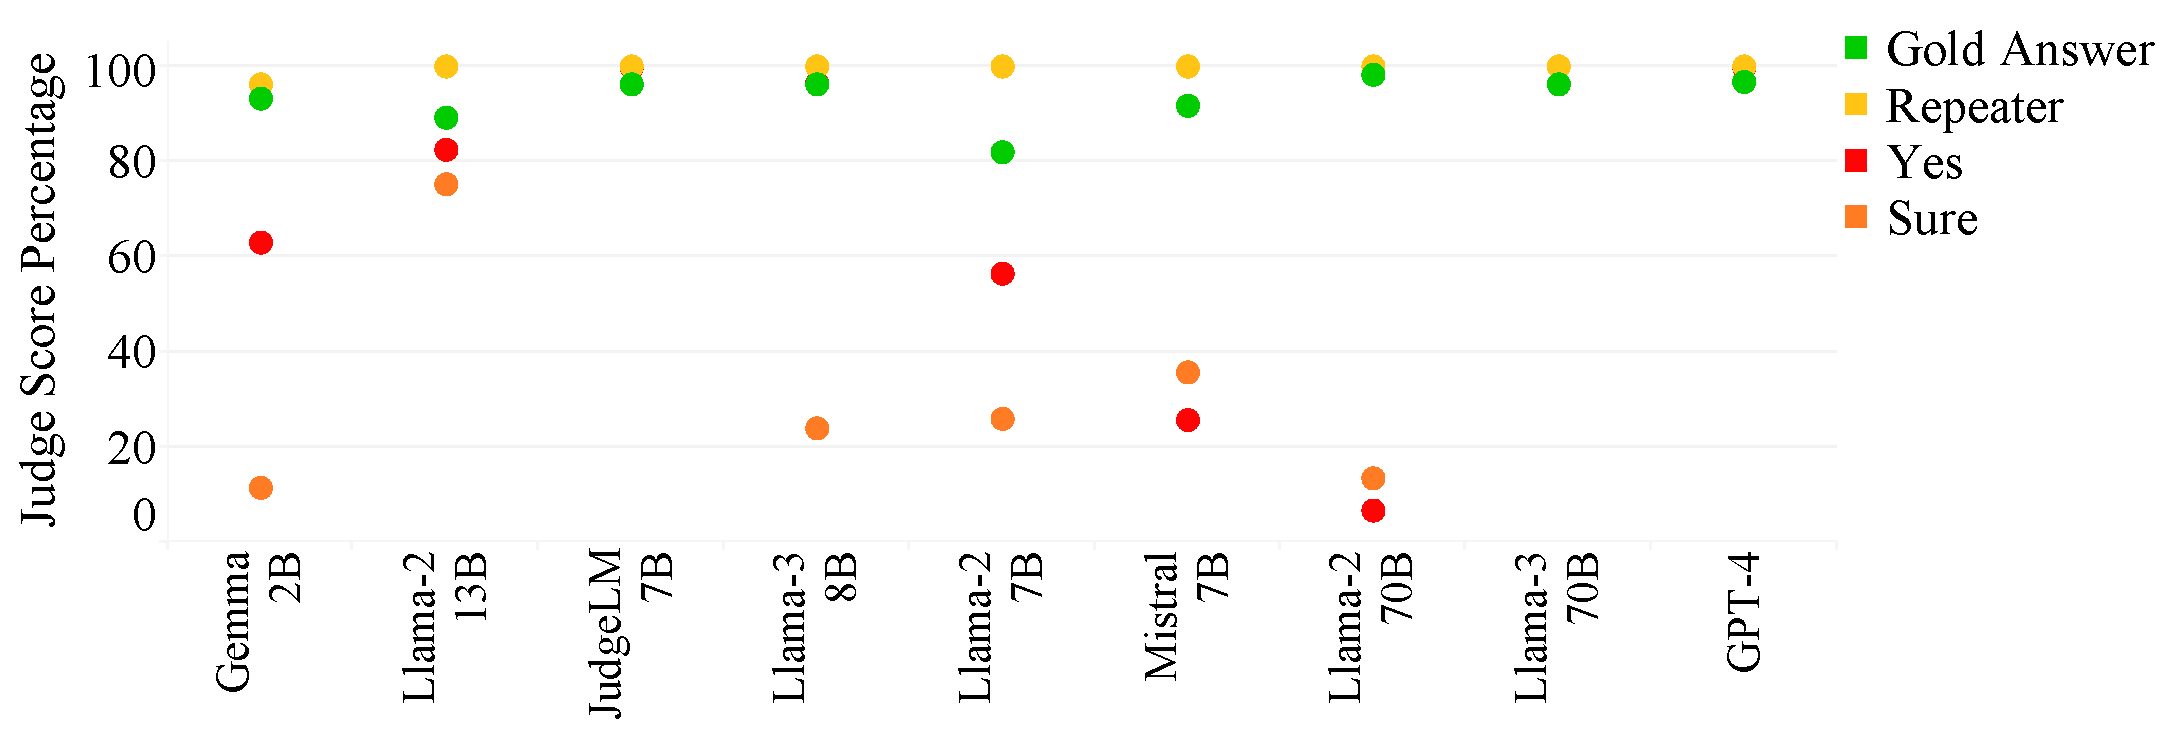
\includegraphics[width=0.825\textwidth]{figures/ConstantV2.pdf}
    \caption{\textbf{Judge responses to dummy answers.} 
    We investigate how \judgemodels respond to dummy answers.
    % , that either repeat the question, simply say `yes' or `sure' or verbatim match one of the reference answers. 
    \judgemodels remain robust when \evaluatormodels produce responses identical to the prompt (`repeater'), but are less robust when the responses are "Yes" and "Sure". Even when the answer matches one of the reference answers verbatim (`Gold answer'), judges do not always arrive at the correct judgement.
    }
    \label{fig:judge_dummy}
\end{figure*}

\subsection{\Judgemodel sensitivity to prompt length and specificity}
\label{sec:analysis:subsec:instructions}

Next, we investigate how prompt length and specificity affect \judgemodels' inferences to determine whether their performance is influenced by \textit{specificity} of the prompt. We use four prompt versions with varying length and specificity.

The first two prompts (\texttt{Without;guidelines;V1/V2}, 45 and 58 tokens) ask for an evaluation without further details. The longer prompts (\texttt{Guidelines;without;examples} and \texttt{Guidelines;with;examples}, 245 and 301 tokens) provide more elaborate guidance and examples. All prompts are listed in \cref{app:TMI}.

\cref{fig:TooMuchInfo} shows that \judge{\gpt}, \judge{Llama-3;70B}, and \judge{Llama-3.1;70B} exhibit low variance in human agreement as prompt length and specificity increases. Top performers show high alignment with humans even with minimal instructions, while they slightly improve with more detailed prompts. In contrast, other models lose alignment with increased instructions, likely due to difficulty processing complex instructions.

In a follow-up experiment, we investigate the impact of reference order (see \cref{app:ref-bias-exp}). \cref{app:ReferenceBiasExample1} and \cref{app:RefernceBiasExample2} shows that larger models maintain consistent judgments regardless of reference order, while smaller models, except \judge{Mistral;7B}, are more sensitive to it.

% Next, we study the impact of the prompt on the predictions of the \judgemodels, to understand if the success of various \judgemodels is related to the \textit{length} of the prompt, and to study the degree to which the judgments of the \judgemodels change with the \textit{specificity} of the prompt.

% We use four different prompt versions, varying in length and specificity.

% The first two prompts (\texttt{Without\;guidelines\;V1/V2}, 45 and 58 tokens, respectively) simply ask to evaluate the responses, without any further information, while more elaborate guidance and examples are given in the longer prompts (\texttt{Guidelines\;without\;examples} and \texttt{Guidelines\;with\;examples}, 245 and 301 tokens, respectively). 
% All prompts are listed in \cref{app:TMI}. 

% \cref{fig:TooMuchInfo} shows that \judge{\gpt}, \judge{Llama-3\;70B} and \judge{Llama-3.1\;70B} exhibit relatively low variance in their agreement with humans as the level of information and the length of the prompt increases.
% For this task, top performers' (\judge{\gpt}, \judge{Llama-3\;70B} and \judge{Llama-3.1\;70B}) implicit definition of a correct judgment seems well aligned with the provided instructions and thus shows high alignment with humans even if no specific instructions are provided.

% It can also be observed that only top performers appears to benefit from the more detailed instructions, with a slight upward trend, whereas the other models get less aligned with more instructions. This might be due to the less powerful judges not being able to follow many instructions in the prompt at the same time.
% % 
% In a follow-up experiment, we further investigate the impact of the order of the reference answers (for details, we refer to \cref{app:ref-bias-exp}). 
% \cref{fig:consistency} illustrates that larger \judgemodels consistently maintain their judgments regardless of the reference order, whereas smaller models -- with the exception of \judge{Mistral\;7B} -- are more sensitive to the reference order given in the prompt.

\subsection{Evaluating controlled responses}
\label{sec:analysis:subsec:judge-ability}

We conduct simple tests on the \judgemodels by having them evaluate dummy benchmark responses. In the first test, the answer is a verbatim reference from the dataset (always correct). In the next three tests, the answers are incorrect. For the second and third tests, the dummy \evaluatormodel responds with \texttt{``Yes''}, and \texttt{``Sure''} respectively. In the fourth test, the evaluated answer is a repetition of the question.

% Next, we perform simple tests on the \judgemodels by asking them to evaluate a set of dummy benchmark responses. For the first test, the answer to be evaluated for each question is one of the references from the dataset, verbatim (the answer is thus always correct).
% For the next three tests, the answer is always incorrect.
% In the second and third tests, the dummy \evaluatormodel always responds with \texttt{``Yes''}, and \texttt{``Sure''} for the second and third tests, respectively.
% For the fourth test, the evaluated answer is a repetition of the question.

% the answer to be evaluated is always incorrect, with the dummy \evaluatormodel always responding with \texttt{``Yes''}, and \texttt{``Sure''} for the 2nd and the 3rd tests, respectively, and simply repeating the question for the fourth test.
%

In \cref{fig:judge_dummy}, we observe that while some \judgemodels correctly identify and mark answers as correct (first test) or incorrect (next three tests), others, like \judge{Llama-2;70B}, incorrect evaluate many dummy answers, despite showing high human alignment on benchmark evaluations (see \cref{fig:llmalignment_b}). We hypothesize that when the answers are plausible but incorrect, judges can correctly identify them as wrong by comparing them with the reference. However, when the answer is unrelated (e.g., \texttt{``Yes''}, and \texttt{``Sure''}), \judgemodels may mistakenly mark them as correct, though further research is needed to clarify this behavior.

% In \cref{fig:judge_dummy}, we can see that while some \judgemodels are able to identify and correctly mark the answers as correct (for the first test) or incorrect (for the next three tests), some judges, notably \judge{Llama-2\;70B}, incorrectly evaluate a significant number of dummy answers, even though they show a relatively high alignment with humans on the benchmark evaluations (see \cref{fig:llmalignment_b}).
% % 
% We hypothesise that when the answers are plausible but incorrect (e.g.\ if the question asks about the name of the author of a book, and the \evaluatormodel gives the name of the wrong author), most judges are able to identify them as being incorrect (by comparing it with the reference answer). 
% However, the judges might get confused about what they are supposed to evaluate if the answer is completely unrelated to the question (such as the words \texttt{``Yes''} and \texttt{``Sure''}). 
% It is possible that, in this situation, a \judgemodel tries to evaluate one of the reference answers, thus marking it as correct, though further research is required to identify the cause of this behavior.



% \begin{figure}[H]
%     \begin{minipage}[b]{0.49\textwidth}
%         \centering
%         \includegraphics[width=\textwidth]{figures/BasevsChat7b.png}
%         % \caption{Comparison Scores for Llama 7B Base and Llama 7B Chat}
%     \end{minipage}
%     \hfill
%     \begin{minipage}[b]{0.49\textwidth}
%         \centering
%         \includegraphics[width=\textwidth]{figures/BasevsChat70b.png}
%         % \caption{Comparison Scores for Llama 70B Base and Llama 70B Chat}
%     \end{minipage}
%     \caption{Comparison of Llama 7B and Llama 70B Models}
%     \label{fig:comparison}
% \end{figure}



% From these observations, we can draw the conclusions that

% 1) There is a knowledge gap between base and chat models which gets more prominent in bigger models. \\
% 2) The ideal LLM evaluator is more lenient than the smaller models and more stricter than GPT \\
% 3) Base models are subject to more relaxed judgement as compared to Chat models.

\subsection{Leniency bias in \judgemodels}
\label{sec:leniency-bias}

% \begin{table}[t]
%     \centering
%     \begin{tabular}{lrrr}
    
%       \toprule
%       Evaluator & $\kappa$ & $P_e$ & $P_+$ \\
%       \midrule
%       Gemma 2B & 0.50 & 0.62 & 0.80 \\
%       Llama-2 7B & 0.66 & 0.68 & 0.36 \\
%       Mistral 7B & 0.72 & 0.75 & 0.75 \\
%       Llama-2 13B & 0.68 & 0.76 & 0.45 \\
%       Llama-2 70B & 0.80 & 0.79 & 0.94 \\
%       Llama-3 8B & 0.81 & 0.80 & 0.84 \\
%       Llama-3 70B & 0.84 & 0.84 & 0.79 \\
%       GPT-4 Turbo & 0.85 & 0.85 & 0.66 \\
%       \bottomrule
% \end{tabular}
% \caption{Estimated values of $P_e$ and $P_+$ for different \judgemodels}
% \label{tab:leniency-bias}
% \end{table}

Lastly, to get a general sense of the inherent biases or misalignment in the evaluation criteria that might be present in the judge models, we estimate if they have a positive or negative bias in their judgment.
To do so, we assume that a judge assigns the correct judgment (i.e.\ same evaluation as the ground truth) with a probability of $P_c$ and assigns the rest of the samples to be \texttt{``correct''} with a probability $P_+$, which we call their \textit{leniency bias}.
% present a crude but simple hypothesis: for a given \judgemodel and a given benchmark, the proportion of times where the evaluation criteria of the \judgemodel align with the provided instructions is given by $P_e$. 
% In the cases where the \judgemodel is not able to correctly understand the task or is not capable enough to evaluate according to the given criteria, it randomly gives an evaluation of \texttt{true} with probability $P_+$, and an evaluation of \texttt{false} with the remaining probability of $1-P_+$, independently of the correctness of the answer.
We estimate the values of $P_c$ and $P_+$ from the benchmark results\footnote{
The theoretical derivation of the expressions for $P_c$ and $P_+$, as well as the empirical validation for their estimated values can be found in \cref{app:leniency-bias}.}
and show them in \cref{tab:p-vals-full}. 
We observe that $P_+$ for most models is significantly higher than $0.5$ (\cref{fig:k-p-corr}), indicating a tendency of the \judgemodels to evaluate responses as \texttt{``correct''} when their evaluation criteria are not completely aligned with the provided instructions. 
